% Quadratic shape functions along one element edge, parametrized by s in [0, 1] (end nodes at s = 0
% and s = 1, mid-edge node at s = 1/2): Lagrange (nodal) versus Bernstein. Both span the same
% quadratic space; only the Bernstein functions are non-negative.
\pgfplotsset{
    shapeaxis/.style={
            width=0.9\linewidth,
            height=0.65\linewidth,
            xmin=0, xmax=1,
            ymin=-0.25, ymax=1.05,
            xlabel={$s$},
            grid=major,
            legend cell align=left,
            legend style={font=\scriptsize},
            legend pos=north east,
        },
    shapeend/.style={blue, line width=1.2pt, domain=0:1, samples=100},
    shapeend2/.style={red, line width=1.2pt, domain=0:1, samples=100},
    shapemid/.style={black, line width=1.2pt, dashed, domain=0:1, samples=100},
}
\begin{figure}[htbp]
    \centering
    \begin{subfigure}[t]{0.48\textwidth}
        \centering
        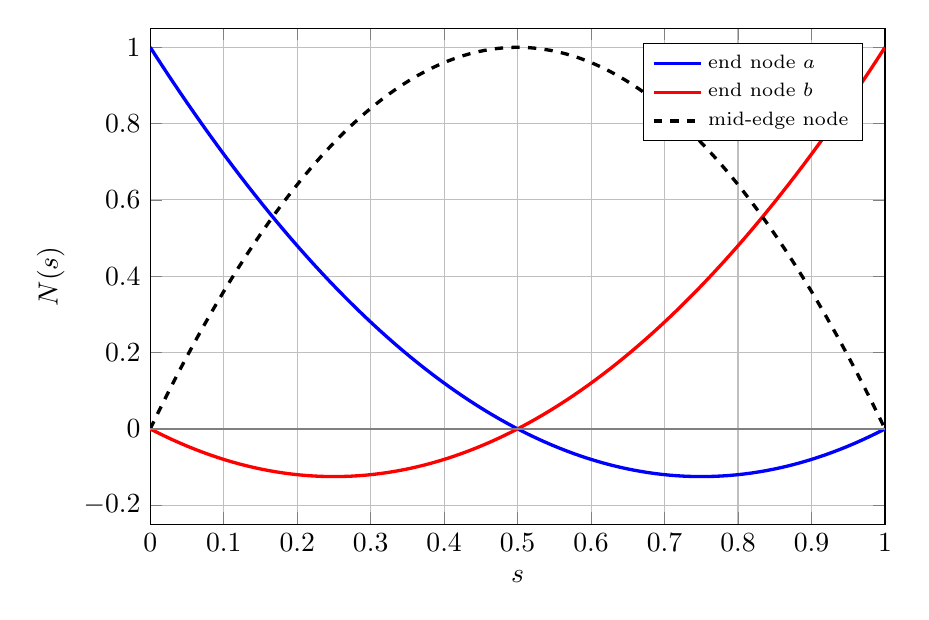
\begin{tikzpicture}
            \begin{axis}[shapeaxis, ylabel={$N(s)$}]
                \addplot[shapeend] {(1-x)*(1-2*x)};
                \addlegendentry{end node $a$}
                \addplot[shapeend2] {x*(2*x-1)};
                \addlegendentry{end node $b$}
                \addplot[shapemid] {4*x*(1-x)};
                \addlegendentry{mid-edge node}
                \addplot[gray, line width=0.6pt, domain=0:1] {0};
            \end{axis}
        \end{tikzpicture}
        \caption{Quadratic Lagrange}\label{fig:shape_lagrange}
    \end{subfigure}
    \hfill
    \begin{subfigure}[t]{0.48\textwidth}
        \centering
        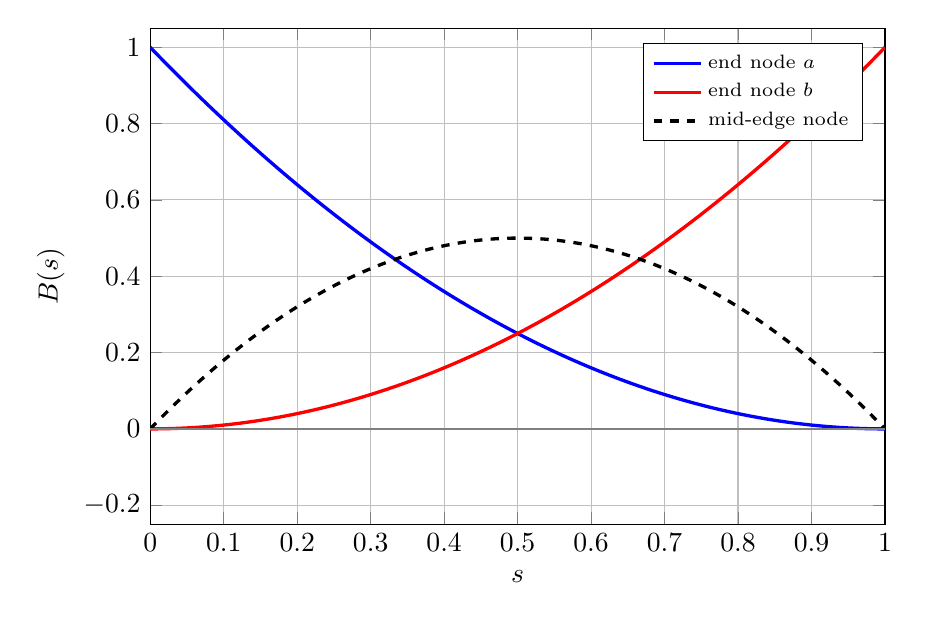
\begin{tikzpicture}
            \begin{axis}[shapeaxis, ylabel={$B(s)$}]
                \addplot[shapeend] {(1-x)^2};
                \addlegendentry{end node $a$}
                \addplot[shapeend2] {x^2};
                \addlegendentry{end node $b$}
                \addplot[shapemid] {2*x*(1-x)};
                \addlegendentry{mid-edge node}
                \addplot[gray, line width=0.6pt, domain=0:1] {0};
            \end{axis}
        \end{tikzpicture}
        \caption{Quadratic Bernstein}\label{fig:shape_bernstein}
    \end{subfigure}
    \caption{Quadratic shape functions along an element edge. The Lagrange end-node functions are negative over half of the edge, so bounds on the nodal values do not bound the field between the nodes. The Bernstein functions are non-negative and sum to one, so the field always lies between the smallest and largest coefficient.}\label{fig:shape_functions}
\end{figure}
